\begin{figure*}[tbp]
\centering
\setlength{\tabcolsep}{3pt}
\begin{tabular}{cccc}
\begin{minipage}[t]{0.22\textwidth}\centering
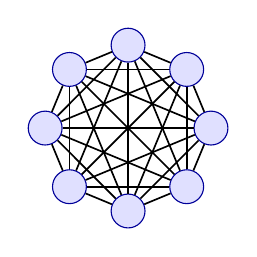
\begin{tikzpicture}[scale=0.78, every node/.style={circle,draw,fill=white,inner sep=1.3pt,minimum size=4.3mm,font=\scriptsize},
edge/.style={line width=0.6pt}, hl/.style={fill=blue!12,draw=blue!60!black}]
  \foreach \i/\ang in {1/90,2/45,3/0,4/315,5/270,6/225,7/180,8/135}{
    \node[hl] (n\i) at (\ang:1.35) {};
  }
  \foreach \i/\j in {1/2,1/3,1/4,1/5,1/6,1/7,1/8,2/3,2/4,2/5,2/6,2/7,2/8,3/4,3/5,3/6,3/7,3/8,4/5,4/6,4/7,4/8,5/6,5/7,5/8,6/7,6/8,7/8}{
    \draw[edge] (n\i)--(n\j);
  }
\end{tikzpicture}
\par\vspace{1mm}\scriptsize \textbf{(a) Global-best}
\end{minipage}
&
\begin{minipage}[t]{0.22\textwidth}\centering
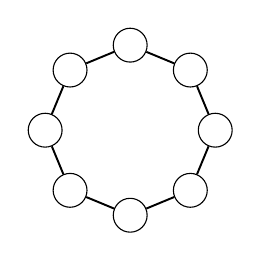
\begin{tikzpicture}[scale=0.8, every node/.style={circle,draw,fill=white,inner sep=1.3pt,minimum size=4.3mm,font=\scriptsize}, edge/.style={line width=0.7pt}]
  \foreach \i/\ang in {1/90,2/45,3/0,4/315,5/270,6/225,7/180,8/135}{
    \node (n\i) at (\ang:1.35) {};
  }
  \foreach \i/\j in {1/2,2/3,3/4,4/5,5/6,6/7,7/8,8/1}{\draw[edge] (n\i)--(n\j);}  
\end{tikzpicture}
\par\vspace{1mm}\scriptsize \textbf{(b) Ring}
\end{minipage}
&
\begin{minipage}[t]{0.22\textwidth}\centering
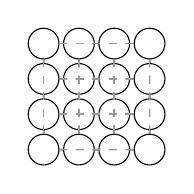
\begin{tikzpicture}[scale=0.66, every node/.style={circle,draw,fill=white,inner sep=1.0pt,minimum size=3.9mm,font=\scriptsize}, edge/.style={line width=0.6pt}, wrap/.style={line width=0.6pt,dashed,gray!80}]
  \foreach \r in {1,2,3,4}{
    \foreach \c in {1,2,3,4}{
      \pgfmathtruncatemacro{\id}{4*(\r-1)+\c}
      \node (n\id) at (0.68*\c, -0.68*\r) {};
    }
  }
  \foreach \r in {1,2,3,4}{
    \foreach \c in {1,2,3,4}{
      \pgfmathtruncatemacro{\cn}{mod(\c,4)+1}
      \pgfmathtruncatemacro{\a}{4*(\r-1)+\c}
      \pgfmathtruncatemacro{\b}{4*(\r-1)+\cn}
      \ifnum\c<4 \draw[edge] (n\a)--(n\b); \else \draw[wrap] (n\a)--(n\b); \fi
    }
  }
  \foreach \c in {1,2,3,4}{
    \foreach \r in {1,2,3,4}{
      \pgfmathtruncatemacro{\rn}{mod(\r,4)+1}
      \pgfmathtruncatemacro{\a}{4*(\r-1)+\c}
      \pgfmathtruncatemacro{\b}{4*(\rn-1)+\c}
      \ifnum\r<4 \draw[edge] (n\a)--(n\b); \else \draw[wrap] (n\a)--(n\b); \fi
    }
  }
\end{tikzpicture}
\par\vspace{1mm}\scriptsize \textbf{(c) Griglia von Neumann toroidale}
\end{minipage}
&
\begin{minipage}[t]{0.22\textwidth}\centering
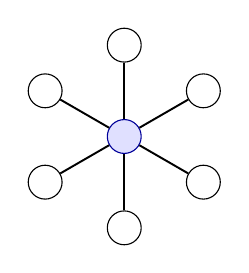
\begin{tikzpicture}[scale=0.8, every node/.style={circle,draw,fill=white,inner sep=1.3pt,minimum size=4.3mm,font=\scriptsize}, edge/.style={line width=0.7pt}, hub/.style={fill=blue!12,draw=blue!60!black}]
  \node[hub] (c) at (0,0) {};
  \foreach \i/\ang in {1/90,2/30,3/330,4/270,5/210,6/150}{
    \node (n\i) at (\ang:1.45) {};
    \draw[edge] (c)--(n\i);
  }
\end{tikzpicture}
\par\vspace{1mm}\scriptsize \textbf{(d) Wheel nell'API (hub-and-spoke)}
\end{minipage}
\\[1.8ex]
\begin{minipage}[t]{0.22\textwidth}\centering
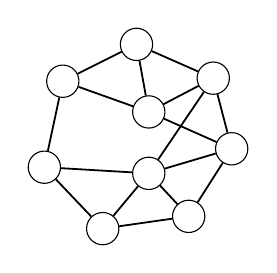
\begin{tikzpicture}[scale=0.78, every node/.style={circle,draw,fill=white,inner sep=1.1pt,minimum size=4.1mm,font=\scriptsize}, edge/.style={line width=0.65pt}]
  \foreach \i/\x/\y in {1/0/1.55,2/1.25/1.0,3/1.55/-0.15,4/0.85/-1.25,5/-0.55/-1.45,6/-1.5/-0.45,7/-1.2/0.95,8/0.2/0.45,9/0.2/-0.55}{
    \node (n\i) at (\x,\y) {};
  }
  \foreach \i/\j in {1/2,1/8,1/7,2/3,2/8,2/9,3/8,3/9,3/4,4/5,4/9,5/6,5/9,6/7,6/9,7/8}{\draw[edge] (n\i)--(n\j);}  
\end{tikzpicture}
\par\vspace{1mm}\scriptsize \textbf{(e) Random connessa, $k\approx4$}
\end{minipage}
&
\begin{minipage}[t]{0.22\textwidth}\centering
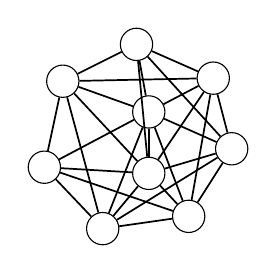
\begin{tikzpicture}[scale=0.78, every node/.style={circle,draw,fill=white,inner sep=1.1pt,minimum size=4.1mm,font=\scriptsize}, edge/.style={line width=0.62pt}]
  \foreach \i/\x/\y in {1/0/1.55,2/1.25/1.0,3/1.55/-0.15,4/0.85/-1.25,5/-0.55/-1.45,6/-1.5/-0.45,7/-1.2/0.95,8/0.2/0.45,9/0.2/-0.55}{
    \node (n\i) at (\x,\y) {};
  }
  \foreach \i/\j in {1/2,1/3,1/7,1/8,1/9,2/3,2/4,2/7,2/8,2/9,3/4,3/5,3/8,3/9,4/5,4/6,4/8,4/9,5/6,5/7,5/8,5/9,6/7,6/8,6/9,7/8,7/9,8/9}{\draw[edge] (n\i)--(n\j);}  
\end{tikzpicture}
\par\vspace{1mm}\scriptsize \textbf{(f) Random connessa, $k\approx8$}
\end{minipage}
&
\begin{minipage}[t]{0.22\textwidth}\centering
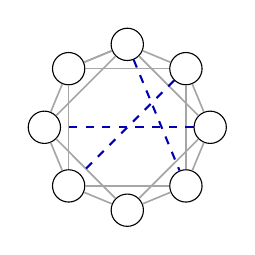
\begin{tikzpicture}[scale=0.78, every node/.style={circle,draw,fill=white,inner sep=1.1pt,minimum size=4.1mm,font=\scriptsize}, edge/.style={line width=0.6pt}, shortcut/.style={line width=0.75pt,blue!70!black,dashed}]
  \foreach \i/\ang in {1/90,2/45,3/0,4/315,5/270,6/225,7/180,8/135}{\node (n\i) at (\ang:1.35) {};}
  \foreach \i/\j in {1/2,2/3,3/4,4/5,5/6,6/7,7/8,8/1,1/8,1/3,2/4,3/5,4/6,5/7,6/8,7/1,8/2}{\draw[edge,gray!70] (n\i)--(n\j);} 
  \foreach \i/\j in {1/4,2/6,3/7}{\draw[shortcut] (n\i)--(n\j);}  
\end{tikzpicture}
\par\vspace{1mm}\scriptsize \textbf{(g) Small-world, $k=4$}
\end{minipage}
&
\begin{minipage}[t]{0.22\textwidth}\centering
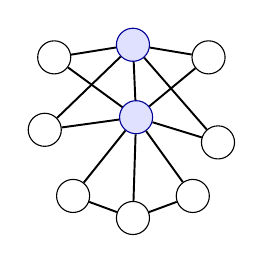
\begin{tikzpicture}[scale=0.8, every node/.style={circle,draw,fill=white,inner sep=1.1pt,minimum size=4.2mm,font=\scriptsize}, edge/.style={line width=0.7pt}, hub/.style={fill=blue!12,draw=blue!60!black}]
  \node[hub] (h1) at (0,1.2) {};
  \node[hub] (h2) at (0.05,0.05) {};
  \node (n3) at (-1.25,1.0) {};
  \node (n4) at (1.2,1.0) {};
  \node (n5) at (-1.4,-0.15) {};
  \node (n6) at (1.35,-0.35) {};
  \node (n7) at (-0.95,-1.2) {};
  \node (n8) at (0.95,-1.2) {};
  \node (n9) at (0,-1.55) {};
  \foreach \i/\j in {h1/h2,h1/n3,h1/n4,h1/n5,h1/n6,h2/n3,h2/n4,h2/n5,h2/n6,h2/n7,h2/n8,h2/n9,n7/n9,n8/n9}{\draw[edge] (\i)--(\j);}  
\end{tikzpicture}
\par\vspace{1mm}\scriptsize \textbf{(h) Scale-free, $k=4$}
\end{minipage}
\end{tabular}
\caption{Schemi TikZ delle otto topologie di comunicazione discusse nel manoscritto. I pannelli sono rappresentazioni qualitative della struttura del vicinato e non corrispondono alla dimensione reale dello sciame usata negli esperimenti. Per le topologie random, small-world e scale-free si mostrano realizzazioni esemplificative; la topologia \texttt{wheel} implementata nel codice coincide con una struttura hub-and-spoke, cio\`e una stella, e non con la wheel grafica standard dotata di anello periferico. Nella griglia von Neumann le linee tratteggiate indicano i collegamenti periodici della topologia toroidale.}
\label{fig:topology-schematics}
\end{figure*}